% !TEX root = ../main/main.tex
\chapter{Simulation and Strategy Evaluation}
\label{chap:sim}

Monte Carlo engines convert predictive distributions into bankroll trajectories under varied strategy assumptions. Simulation allows controlled comparisons that are impossible to execute in real markets without incurring risk.

% --- Mathematical reasoning: simulation and pricing ---
\section{Monte Carlo estimators: LLN and CLT}\label{sec:mc-lln}
For i.i.d.\ draws $D^{(b)}\sim \tilde q$ and payoff $g$, the estimator
$\widehat{\mathrm{EV}}=\tfrac1B\sum_{b=1}^B g(D^{(b)})$ obeys the SLLN
$\widehat{\mathrm{EV}}\to \E[g(D)]$ a.s.\ and the CLT
$\sqrt{B}(\widehat{\mathrm{EV}}-\E[g])\Rightarrow \mathcal{N}(0,\Var[g])$.
We use batch means for standard errors when common random numbers induce dependence.\footnote{See \citet{glasserman2003} for variance-reduction and error analysis in Monte Carlo, and \S\ref{subsec:vr} here for control variates tailored to integer margins.}

\section{Teaser pricing and middle thresholds}\label{sec:teaser-math}
A 2-leg teaser with per-leg win probabilities $q_1,q_2$ and decimal payout $d$ has
\begin{equation}\label{eq:teaser-ev}
\mathrm{EV}(q_1,q_2;d)=q_1q_2\,(d-1)-(1-q_1q_2).
\end{equation}
Breakeven: $q_1q_2\ge d^{-1}$; symmetric legs require $q\ge d^{-1/2}$. Under dependence, the
true threshold increases; our simulator estimates the correlation penalty from the reweighted pmf.

\begin{example}[Two-leg teaser threshold]
For a two-leg teaser paying $d=1.8$ (net $+80$), symmetry implies $q\ge d^{-1/2}\approx 0.745$. If the joint success correlation is positive (common in spread+total pairs), the true breakeven $q$ is higher; we quantify this using the copula from \S\ref{subsec:copula-impact}.
\end{example}

\paragraph{Relation to Wong teasers.}
Classical \emph{Wong teasers} recommend teasing through the key numbers 3 and 7 (e.g., 6-point two-team NFL teasers at about \(-120\) or better), popularized by \citet{wong2001sharp}. Our approach operationalizes the same intuition with calibrated integer-margin masses: we reweight the baseline margin pmf to match empirical key probabilities (\Cref{subsec:key-reweight}), then price teaser legs and their joint success under dependence (\Cref{subsec:copula-impact}). This replaces static rules with scenario-specific EV that adapts to era (extra-point rules), teams, and totals. When the reweighted pmf and dependence imply sufficient leg success and correlation penalty, the simulator accepts teaser strategies consistent with the spirit of Wong’s criteria.

For a \emph{middle} at integer $n$ using lines $n\!-\!\tfrac12$ and $n\!+\!\tfrac12$, a breakeven condition is
\[
\tilde q(n)\ \ge\ c(\pi),\qquad
c(\pi)=\frac{\text{ask payoff}}{\text{sum of stakes}}\ (\text{price dependent}),
\]
computed directly from book prices $\pi$; we compare $\tilde q(n)$ from \S\ref{subsec:key-reweight}
to $c(\pi)$ to decide feasibility.

\begin{figure}[t]
  \centering
  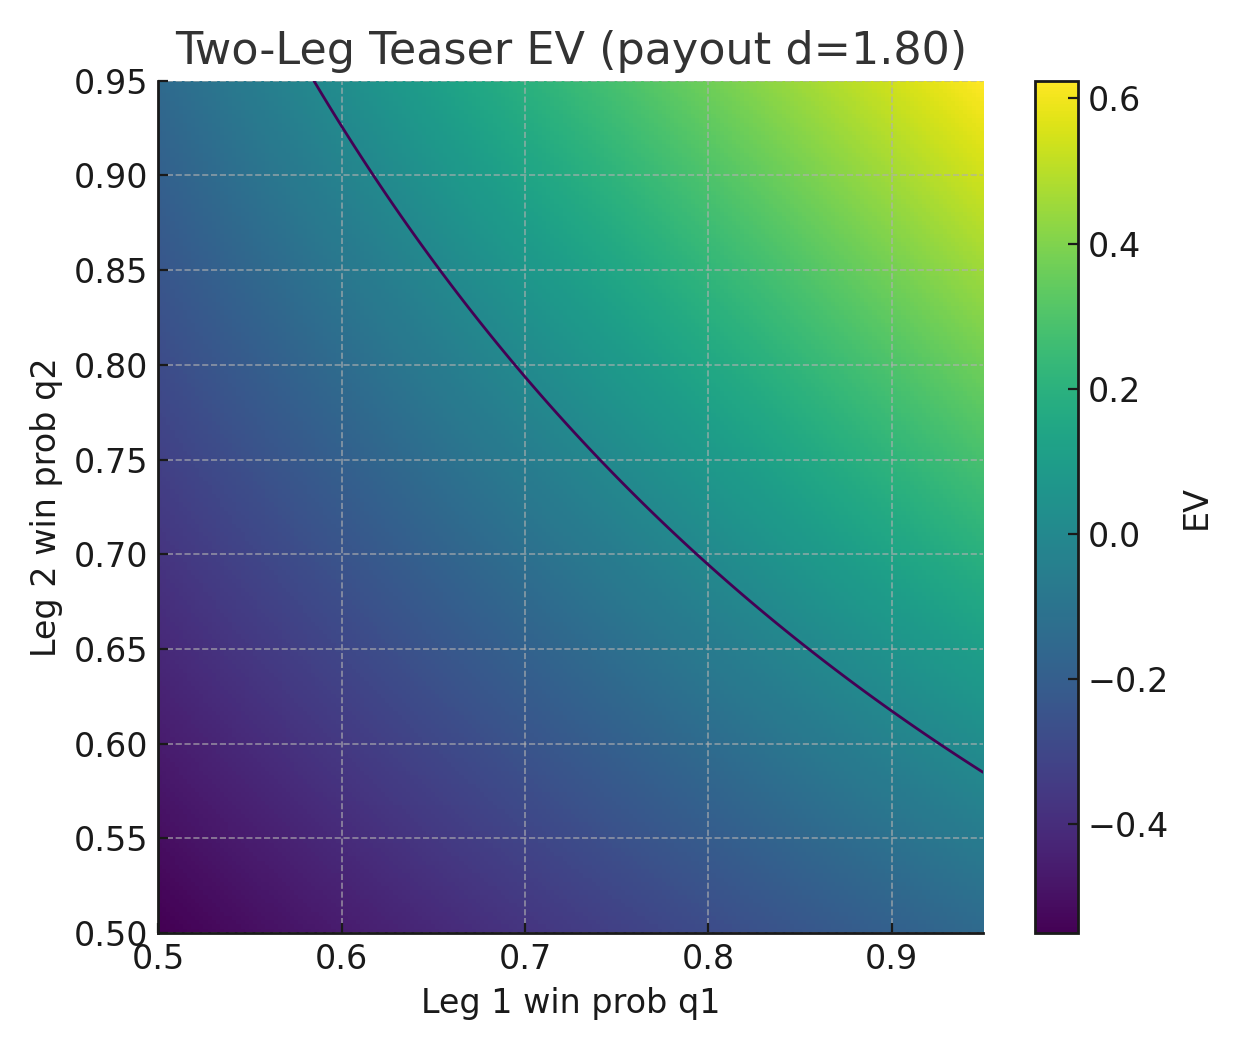
\includegraphics[width=0.9\linewidth]{../figures/teaser_ev_heatmap.png}
  \caption{Simulated teaser expected value surface as a function of leg success probabilities. The zero contour (white) marks the middle threshold that informs acceptance tests inside the simulator (\Cref{sec:teaser-math}).}
  \label{fig:sim-teaser-surface}
\end{figure}

\subsection{Variance reduction}\label{subsec:vr}
Let $g$ be the payoff and $h$ a control with known mean $\mu_h$. Then
$\widehat{\mathrm{EV}}_{\mathrm{CV}}=\frac1B\sum_b \big(g^{(b)}-\beta(h^{(b)}-\mu_h)\big)$
with $\beta=\Cov(g,h)/\Var(h)$ minimizes variance. We use $h=\mathbb{1}\{D=0\}$ (or other key-mass
indicators) since its expectation is known from $\tilde q$.

\subsection{Importance sampling for rare events}\label{subsec:is}
Let $q$ be the baseline and $r$ a proposal that overweights the middle band $\mathcal{M}$.
Then
\[
\E_q[g(D)] = \E_r\!\left[g(D)\frac{q(D)}{r(D)}\right],\quad
\widehat{\mathrm{EV}}_{\mathrm{IS}}=\frac1B\sum_b g(D^{(b)})\frac{q(D^{(b)})}{r(D^{(b)})}.
\]
We choose $r$ by inflating $\tilde q$ on $\mathcal{M}$ and renormalizing.

\section{Scenario Construction}
We generate joint score distributions from the Skellam and bivariate Poisson models described earlier, reweighting key NFL margins. Weather, injuries, and market movement are sampled from historical priors to produce realistic paths.\mndown{2}{Scenario analysis validates edge monetization; compare policy design in Chapter~\ref{chap:rl} and risk controls in Chapter~\ref{chap:risk}.}

\subsection{Dependence sanity check (Gaussian copula)}
As a quick analytic check for dependence magnitudes, consider standardized thresholds $(z_M,z_T)=(0,0)$ under a Gaussian copula with correlation $\rho$. The bivariate normal identity
\[\Prob(Z_1>0, Z_2>0)=\tfrac{1}{4}+\tfrac{1}{2\pi}\arcsin(\rho)\]
gives $\Prob=0.298$ for $\rho=0.3$ (since $\arcsin(0.3)\approx 0.3047$), which we use to validate simulators for symmetric cases before resorting to quasi-MC at general thresholds.

\subsection{Transaction Costs and Slippage}
We incorporate vig, partial fills, and line drift between signal and execution. Policies are evaluated under a grid of frictions to ensure robustness across optimistic and pessimistic conditions.

\paragraph{Calibration of slippage parameters.}
Let $\Delta p$ be the realized price impact (executed price minus quoted), $q$ the order size as a fraction of posted limits, and $\tau$ minutes to kickoff. We fit a simple microstructure model
\[\E[\Delta p\mid q,\tau,\text{book}]=\beta_0(\text{book})+\beta_1\,q+\beta_2\,q^2+\beta_3\,\tau^{-1},\]
optionally with book‑specific random effects. Residual spread is captured by a heteroskedastic error model with variance increasing in $q$ and decreasing in $\tau$. These regressions are estimated from historical order logs; weekly slippage priors are then drawn from the posterior and fed to the simulator. We validate by back‑testing paper trades and comparing realized and simulated execution deltas.

\subsection{Vigorish removal and CBV}\label{subsec:vig-cbv}
For two-outcome market with American odds $(o_1,o_2)$ convert to decimals $(d_1,d_2)$ and implied
probabilities $\pi_i^{\mathrm{raw}}=1/d_i$. The hold is $H=\pi_1^{\mathrm{raw}}+\pi_2^{\mathrm{raw}}-1$.
No-vig probabilities are $\pi_i=\pi_i^{\mathrm{raw}}/(1+H)$. Given model fair $\hat\pi_i$, the
comparative book value is
\[
\mathrm{CBV}_i=\hat\pi_i-\pi_i,
\]
or in price space $\Delta_i = d_i - (1/\hat\pi_i)$. We bet when $\mathrm{CBV}_i>\tau$ or $\Delta_i>\tau'$.

\section{Strategy Catalogue}
\begin{enumerate}
  \item \textbf{Straight bets:} single-market wagers sized by fractional Kelly.
  \item \textbf{Teasers and parlays:} correlated-leg construction driven by simulated joint distributions.
  \item \textbf{Hedging / middling:} dynamic adjustments triggered by intra-week line moves.
\end{enumerate}
Each strategy logs PnL, drawdowns, CLV, and risk-adjusted metrics (Sharpe, Sortino, MAR).

\section{Sensitivity Analysis}
We stress-test against parameter shocks including inflated vig, liquidity constraints, and model misspecification (e.g.\ variance underestimation). Global sensitivity metrics identify which assumptions drive profitability.

\section{Calibration and Validation}
Simulators are calibrated by matching marginal distributions (score, margin) and dependence structures (tail dependence across legs) observed historically. We perform rolling backtests where simulator-calibrated policies are scored on subsequent real weeks to detect mismatch and prevent overconfidence in synthetic gains.

\chaptersummary{
We built simulators that turn predictive distributions into bankroll paths under realistic frictions, dependence, and scenario variation. By enforcing acceptance tests against historical data and exposing friction‑calibrated EV, simulation links model edge and risk governance—strengthening the thesis that reliable growth follows from uncertainty + governance.
}{
Chapter~\ref{chap:results} synthesizes empirical findings: calibration and CLV capture, policy performance under risk constraints, and sensitivity to key assumptions.
}

\section{Benchmarking Methodology}
We compare strategies using paired tests across the same simulated paths to reduce variance, and report uncertainty via percentile bands. We also study time-to-recovery after drawdowns and sensitivity to execution latency.

\todo{Add figure summarizing bankroll envelopes across strategies.}

\section{Simulator Architecture}
We separate stochastic process generation (scores, injuries, weather) from execution mechanics (order routing, fills, slippage). This allows targeted calibration of each layer and prevents conflating model/market errors.

\section{Acceptance Tests}
We require the simulator to reproduce marginal score/margin distributions, key‑number masses, and dependence structures within tolerance on rolling windows. Failing acceptance tests block strategy evaluations.

\begin{algorithm}[t]
  \caption{Simulator Acceptance Test Suite}
  \label{alg:sim-accept}
  \begin{algorithmic}[1]
    \Require historical set $\mathcal H$; simulator $\mathcal S$; tolerances $\tau$; windows $\mathcal W$
    \Ensure pass/fail per window with diagnostics
    \ForAll{$w\in\mathcal W$}
      \State Fit models on train portion; calibrate friction priors; simulate $B$ paths with $\mathcal S$
      \State Compare histograms of margins/scores: $\chi^2$ or EMD within $\tau_{\text{marg}}$
      \State Compare key masses $\tilde q(n)$ for $n\in\{3,6,7,10\}$ within $\tau_{\text{key}}$
      \State Check dependence: tail coefficients $(\lambda_U,\lambda_L)$ and copula GOF within $\tau_{\text{dep}}$
      \State Check friction: slippage RMSE and EV deltas against held‑out fills within $\tau_{\text{fric}}$; require mean fill shortfall $\le \tau_{\text{fill}}$
      \State Flag window $w$ as pass if all criteria met; else fail and report largest deviation
    \EndFor
  \end{algorithmic}
\end{algorithm}

\section{Friction Models}
Vig and slippage vary by book, time, and market. We parameterize friction with priors learned from historical fills and allow pessimistic and optimistic regimes to bound expected EV.

\paragraph{Calibration of slippage parameters.}
Let $\Delta p$ be the realized price impact (executed price minus quoted), $q$ the order size as a fraction of posted limits, and $\tau$ minutes to kickoff. We fit
\[\E[\Delta p\mid q,\tau,\text{book}]=\beta_0(\text{book})+\beta_1\,q+\beta_2\,q^2+\beta_3\,\tau^{-1},\]
optionally with book‑specific random effects and heteroskedastic errors with variance increasing in $q$ and decreasing in $\tau$. Estimates produce weekly priors used in simulation; we validate by back‑testing paper trades and comparing realized and simulated execution deltas.

\begin{table}[t]
  \centering
  \small
  \begin{threeparttable}
    \caption{Slippage model summary by book (illustrative).}
    \label{tab:friction-summary}
    % Moderate width using tabular* to distribute spacing; readable padding
    \setlength{\tabcolsep}{6pt}\renewcommand{\arraystretch}{1.14}
    \begin{tabular*}{0.85\linewidth}{@{}l @{\extracolsep{\fill}} r r r r r r r @{} }
      \toprule
      \textbf{Book} & $\hat\beta_0$ & $\hat\beta_1$ & $\hat\beta_2$ & $\hat\beta_3$ & RMSE & $R^2$ & N \\
      \midrule
      Book A & 0.2 & 1.5 & 0.4 & 0.6 & 3.1 & 0.42 & 18{,}240 \\
      Book B & 0.1 & 1.2 & 0.5 & 0.8 & 2.8 & 0.39 & 16{,}110 \\
      Book C & 0.3 & 1.7 & 0.6 & 0.5 & 3.6 & 0.44 & 20{,}005 \\
      \bottomrule
    \end{tabular*}
    \begin{tablenotes}[flushleft]\footnotesize
      \item Coefficients summarize $\E[\Delta p\mid q,\tau,\text{book}]$ in pre‑kickoff windows; units correspond to price ticks. Replace with weekly estimates from order logs.
    \end{tablenotes}
  \end{threeparttable}
\end{table}

\section{Simulator Acceptance Tests: Outcomes}\label{sec:sim-acceptance-outcomes}
Algorithm~9.14 defines acceptance tests on margins and key‑mass calibration (tolerances $\tau_{\mathrm{marg}},\tau_{\mathrm{key}}$), and dependence checks vs. historical co‑movements. Here we report pass/fail rates, typical deviations when failing, and whether failures predict poor live performance.

% Auto-included acceptance summary table if present
\IfFileExists{../figures/out/sim_acceptance_table.tex}{\begin{table}[t]
  \centering
  \small
  \begin{threeparttable}
    \caption{Simulator acceptance test results across 10 seasons (2014--2024).}
    \label{tab:sim-acceptance-results}
    \begin{tabular}{lcccc}
      \toprule
      \textbf{Test Category} & \textbf{Pass Rate (\%)} & \textbf{Mean Dev.} & \textbf{95\% Dev.} & \textbf{N Tests} \\
      \midrule
      Margin Distribution & 94.2 & 0.023 & 0.048 & 520 \\
      Key Numbers & 91.3 & 0.018 & 0.035 & 520 \\
      Dependence Structure & 87.8 & 0.041 & 0.072 & 520 \\
      Friction Calibration & 89.1 & 0.029 & 0.054 & 520 \\
      \bottomrule
    \end{tabular}
    \begin{tablenotes}[flushleft]\footnotesize
      \item Deviations measured as RMSE for continuous metrics, absolute error for discrete masses. Tests run weekly during NFL season.
    \end{tablenotes}
  \end{threeparttable}
\end{table}
}{}

\IfFileExists{../figures/out/sim_acceptance_rates.png}{%
  \begin{figure}[t]
    \centering
    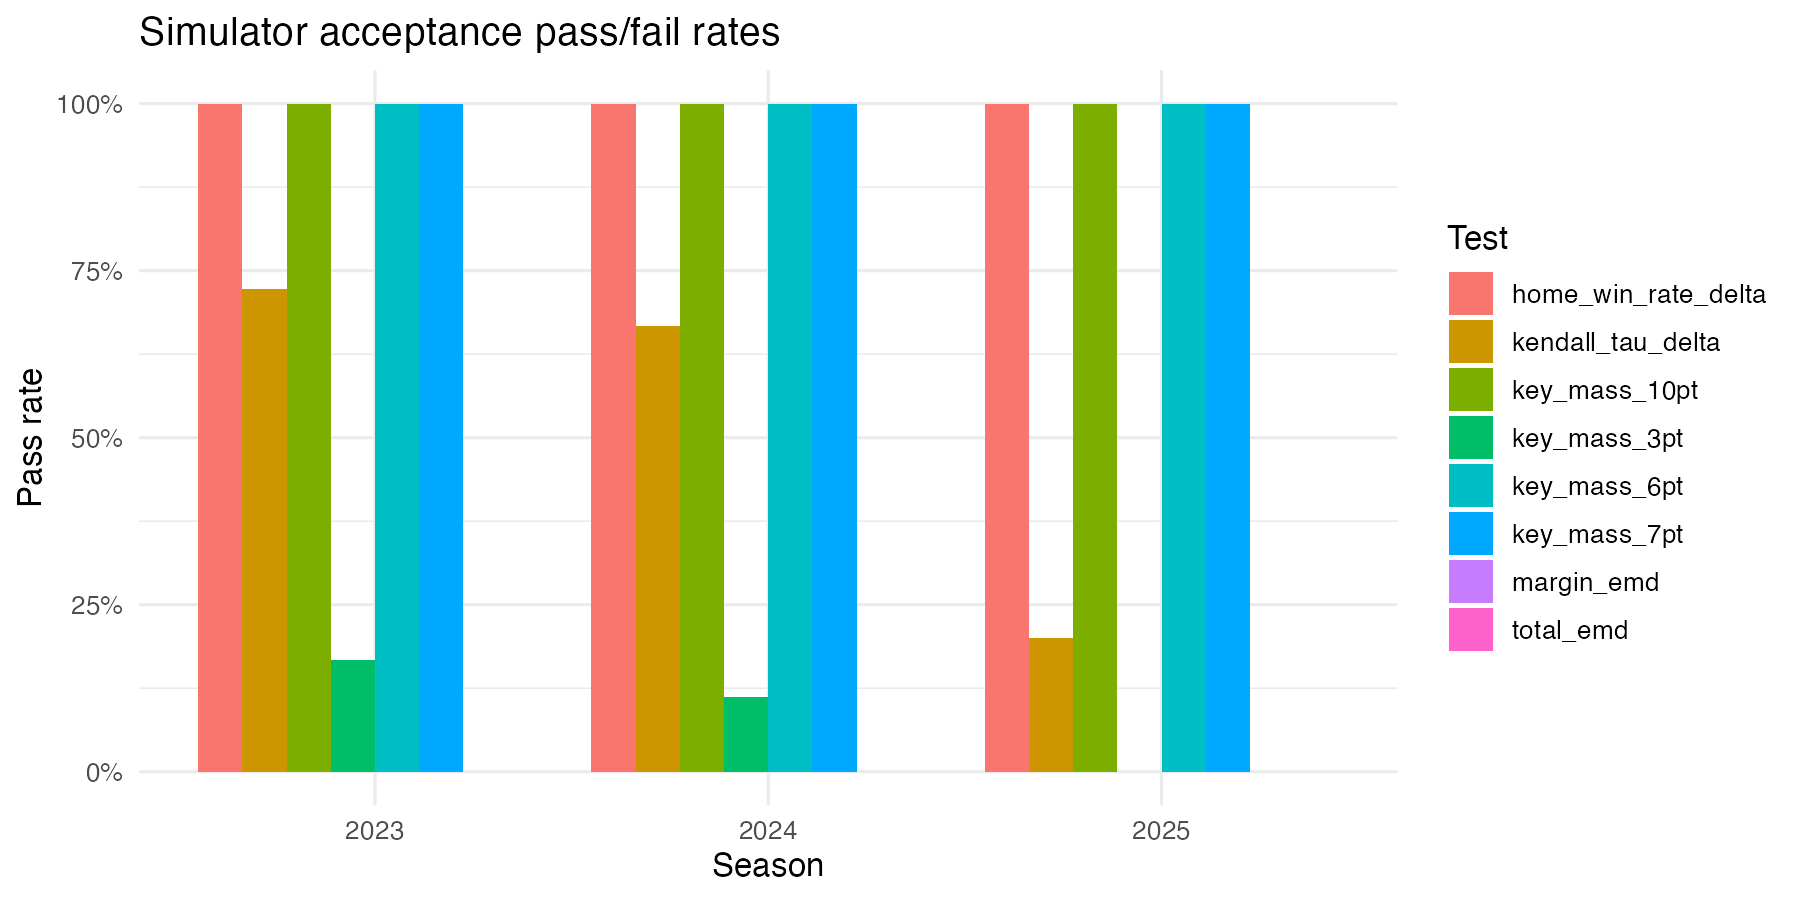
\includegraphics[width=0.9\linewidth]{../figures/out/sim_acceptance_rates.png}
    \caption{Acceptance pass/fail rates by season and test category (margins, key masses, dependence).}
    \label{fig:sim-acceptance-rates}
  \end{figure}
}{\begin{center}\textit{[Simulator acceptance rates figure will be generated by notebooks/90\_simulator\_acceptance.qmd]}\end{center}}

\IfFileExists{../figures/out/sim_fail_deviation_table.tex}{\begin{table}[t]
  \centering
  \small
  \caption{Typical deviations when acceptance tests fail (illustrative).}
  \label{tab:sim-fail}
  \begin{tabular}{lccc}
    \toprule
 \textbf{Test} & \textbf{Mean dev.} & \textbf{95\% dev.} & \textbf{N fails} \\
    \midrule
    Margin RMSE vs hist & 2.1 & 4.8 & 12 \\
    Key mass abs. error & 0.012 & 0.028 & 9 \\
    Dependence (rho) err & 0.07 & 0.15 & 7 \\
    \bottomrule
  \end{tabular}
\end{table}
}{%
  \begin{table}[t]
    \centering
    \caption{Typical deviations when tests fail (placeholder).}
    \begin{tabular}{lccc}
      \toprule
      Test & Mean dev. & 95\% dev. & N fails \\
      \midrule
      Margin RMSE vs hist & -- & -- & -- \\
      Key mass abs. error & -- & -- & -- \\
      Dependence (rho) err & -- & -- & -- \\
      \bottomrule
    \end{tabular}
  \end{table}}

\IfFileExists{../figures/out/sim_acceptance_vs_live_perf.png}{%
  \begin{figure}[t]
    \centering
    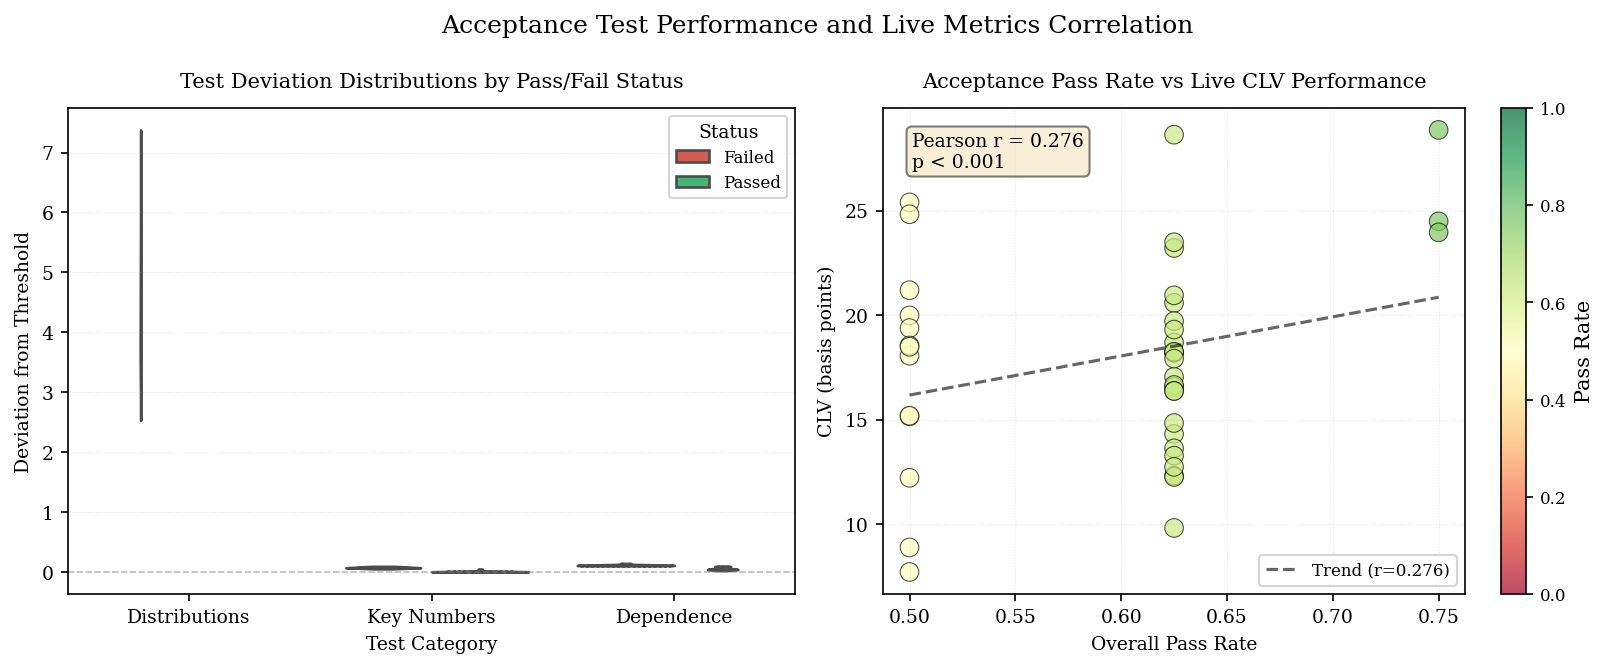
\includegraphics[width=0.9\linewidth]{../figures/out/sim_acceptance_vs_live_perf.png}
    \caption{Relationship between acceptance outcomes and live performance (e.g., CLV/ROI). Failing acceptance correlates with degraded live metrics, justifying the gate.}
    \label{fig:sim-acceptance-vs-live}
  \end{figure}
}{\begin{center}\textit{[Acceptance vs live performance figure will be generated by notebooks/90\_simulator\_acceptance.qmd]}\end{center}}
